%%%%%%%%%%%%%%%%%%%%%%%%%%%%%%%%%%%%%%%%%
% University/School Laboratory Report
% LaTeX Template
% Version 3.1 (25/3/14)
%
% This template has been downloaded from:
% http://www.LaTeXTemplates.com
%
% Original author:
% Linux and Unix Users Group at Virginia Tech Wiki 
% (https://vtluug.org/wiki/Example_LaTeX_chem_lab_report)
%
% License:
% CC BY-NC-SA 3.0 (http://creativecommons.org/licenses/by-nc-sa/3.0/)
%
%%%%%%%%%%%%%%%%%%%%%%%%%%%%%%%%%%%%%%%%%

%----------------------------------------------------------------------------------------
%	PACKAGES AND DOCUMENT CONFIGURATIONS
%----------------------------------------------------------------------------------------

\documentclass{article}

\usepackage[version=3]{mhchem} % Package for chemical equation typesetting
\usepackage{siunitx} % Provides the \SI{}{} and \si{} command for typesetting SI units
\usepackage{graphicx} % Required for the inclusion of images
\usepackage{natbib} % Required to change bibliography style to APA
\usepackage{amsmath} % Required for some math elements 
\usepackage[dvipsnames]{xcolor} % Give colors to text
\usepackage{hyperref}


\setlength\parindent{0pt} % Removes all indentation from paragraphs

\renewcommand{\labelenumi}{\alph{enumi}.} % Make numbering in the enumerate environment by letter rather than number (e.g. section 6)

%\usepackage{times} % Uncomment to use the Times New Roman font


\newcommand{\locx}{\mathbf{x}}
\newcommand{\vele}{\mathbf{e}_\alpha}

\usepackage[margin=0.8in]{geometry}
%----------------------------------------------------------------------------------------
%	DOCUMENT INFORMATION
%----------------------------------------------------------------------------------------

\title{Lattice Boltzmann Method\\ Math, Physics \& Bibliographic Review\\Penn State University} % Title

\author{Nicolás \textsc{Bueno}} % Author name

\date{\today} % Date for the report

\begin{document}
	
	\maketitle % Insert the title, author and date
	
	\begin{center}
		\begin{tabular}{c c}
			Program: & PhD in Energy and Mineral Engineering\\
			Supervisor: & Dr. Ayala\\
			Co-advisor: & Dr. Mehmani
		\end{tabular}
	\end{center}
	
	% If you wish to include an abstract, uncomment the lines below
	 \begin{abstract}
	This text is a personal adjunct to the LBM tutorials to further study some mathematical aspects of the method, open the discussion to physical aspects of the theory, and finally, propose a new Fortran OOP implementation. Bibliographic review to penetrate into possible research directions for my PhD investigation is presented. 
	 \end{abstract}
	
	\tableofcontents
	
	\newpage
	%----------------------------------------------------------------------------------------
	%	SECTION 
	%----------------------------------------------------------------------------------------
	
	\section{LBM Theory}
	
	\subsection{Questions from Tutorial 0}
	\paragraph{Vertical-Horizontal Momentum}
	Why is horizontal momentum converted into vertical momentum in Lattice Gas Automata? I assume that otherwise, molecules could only travel in one direction, restricting the model to represent actual fluids.\\
	
	\textcolor{red}{ANS:}
	
	\paragraph{Figure 8} Is the notation correct here? Let's focus on $f^{\text{in}}_1$ distribution, that comes from left horizontal-moving lattice. Shouldn't it be $f^{\text{in}}_3$, and $f^{\text{in}}_1$ be defined as the particles coming from the right horizontal-moving lattice?\\
	
	\textcolor{red}{ANS:} As each $f_i$ has assigned certain velocity vector, the direction of $f_i$ cannot change, so incoming DF has to come from the opposite side it points to. 
	
	\paragraph{Macroscopic variables from $f^{\text{eq}}$}
	Equations (5) and (6) from Tutorial 1 suggest that density and velocity are obtained from the equilibrium distribution functions as:

	\begin{eqnarray}
		\rho = \sum f^{eq}_i  \\
		\rho \cdot \mathbf{u} = \sum_i f^{eq}_i \cdot  \mathbf{e}_i
	\end{eqnarray}
	
	Although we are assuming near-equilibrium conditions, is it correct to define macroscopic variables as this and not using the actual DFs?\\
	
	\textcolor{red}{ANS:}
	
	\paragraph{About scaling in LBM}
	
	
	\subsection{Questions from Tutorial 1}
	
	\paragraph{Avogadro's number in macroscopic variables} In Equation (1.2) is presented the definition of density using the distribution function $\hat{f}$, which stands for number of molecules per specific molecular velocity and per unit volume. Following this convention, I found a small issue in defining the density as $\rho = M_{w} \int \hat{f} d\pmb{\xi}$, because the final units would be ``number of molecules" times ``mass" per unit volume per unite moles. However, the number of molecules and moles are related through the Avogadro's number, what allows rewriting the equation as:
	\begin{equation}
		\rho = \frac{M_w}{N_A} \int \hat{f} d\pmb{\xi} = \int f d\pmb{\xi}, \, \, \, f=\frac{M_w}{N_A}\hat{f}
	\end{equation}

	\paragraph{``Dilute" concept and Knudsen number} To define a proper collision operator, two assumptions are needed: a) hard spheres collision conserves mass, momentum, and kinetic energy, b) ``dilute" mixture to assure only bi-molecule collisions occur. This paragraph defines again the concept of dilute flow. Dilute has to perspectives: microscopic and macroscopic. The microscopic dilute means that molecule sizes are much smaller than their mean free path (make draw) (although operator can handle dense flow for liquids, incorporating a correction).
	
	The macroscopic dilute is related to the Knudsen number, defines as:
	\begin{equation}
		K_n = \frac{\lambda}{L}
	\end{equation}
	being $\lambda$ the mean free path of molecules, and $L$ the characteristic length of the flow. If $K_n$ < 0.01, a dense flow, the continuum assumption can be applied, supporting the validity of Navier-Stokes' equation and Fourier's law. Microscopic dilute is often applied when working with gases, as statistical mechanics predict mean free paths usually much larger than the molecule sizes. An example of microscopic dilute and macroscopic dense flow is the air flow in a room of few meters (characteristic length), as the mean free path of molecules if much smaller than room size. On the other hand, a microscopic and macroscopic dilute is the air flow through a nanopore or narrow orifice, where the molecules free path is comparable with the size of the pore. 
	
	
	\paragraph{From BGK to LBM} During the development of LBM equations, the starting point was the Boltzmann-BGK equation:
	\begin{equation}
		\frac{\partial f_i}{\partial t} + \pmb{\xi} \frac{\partial f_i}{\partial \mathbf{x}} = -\frac{f_i - f^{\text{eq}}_i}{\tau} - \mathbf{F}_i, \, \, \, \mathbf{F}_i = \mathbf{a} \frac{\partial f_i}{\partial \pmb{\xi}}
	\end{equation}

	That can be discretized as the discrete Boltzmann-BGK equation:
	\begin{equation}
		\frac{\partial f_i}{\partial t} + \mathbf{e_i} \frac{\partial f_i}{\partial \mathbf{x}} = -\frac{f_i - f^{\text{eq}}_i}{\tau} - \mathbf{F}_i, \, \, \, \mathbf{F}_i = \mathbf{a} \frac{\partial f_i}{\partial \mathbf{e_i}}
	\end{equation}
	
	\textcolor{red}{Question}: As the lattice Boltzmann method is divided in two steps (collision and streaming), can we take $\frac{\partial f_i}{\partial \mathbf{x}}$ during collision (``characteristic line" or constant $\mathbf{x}$)?
	
	\textcolor{red}{ANS:}\\
	
	The left-hand side (LHS) temporal term can be discretized as:
	\begin{equation*}
		\frac{\partial f_i}{\partial t} \approx \frac{f^{n+1}_i - f^{n}_i}{\delta t}
	\end{equation*}
	
	The right-hand side (RHS), that has not any temporal derivative, can be discretized in the time domain in several ways. The Crank-Nicholson scheme, which is analog to the trapezoidal rule for the area under the curve, is employed: 
	\begin{equation*}
		-\frac{f_i - f^{\text{eq}}_i}{\tau} - \mathbf{F}_i \approx \frac{1}{2}  \left[ \left( - \frac{f_i - f^{\text{eq}}_i}{\tau} - \mathbf{F}_i \right)^{n} + \left( - \frac{f_i - f^{\text{eq}}_i}{\tau} - \mathbf{F}_i \right)^{n+1} \right]
	\end{equation*}
	
	If we replace both sides, again, for a constant position $\mathbf{x}$, we end up with:
	\begin{equation}\label{eq:originalLBM}
		 \frac{f^{n+1}_i - f^{n}_i}{\delta t}  = \frac{1}{2}  \left[ \left( - \frac{f_i - f^{\text{eq}}_i}{\tau} - \mathbf{F}_i \right)^{n} + \left( - \frac{f_i - f^{\text{eq}}_i}{\tau} - \mathbf{F}_i \right)^{n+1} \right]
	\end{equation}
	
	Let's proceed to become last equation fully explicit by defining a new $\bar{f}$ as:
	\begin{equation}\label{eq:redefineDF}
		\bar{f}_i = f_i + \frac{\delta t}{2\tau} [f_i-f^{\text{eq}}_i] +\frac{\delta t}{2} \mathbf{F}_i
	\end{equation}
	
	Rearranging equation~\ref{eq:originalLBM}, with $n+1$ terms to the left, and $n$ to the right, and defining $\Delta f_i=f_i - f^{\text{eq}}_i$:
	\begin{equation*}
		f^{n+1}_i + \frac{\delta t}{2} \left( \frac{\Delta f_i}{\tau} + \mathbf{F}_i \right)^{n+1} = f^{n}_i + \frac{\delta t}{2} \left( - \frac{\Delta f_i}{\tau} - \mathbf{F}_i \right)^{n}
	\end{equation*}
	LHS of this equation is the definition of $\bar{f}^{n+1}_i$, and if we solve for $f_i$ in equation~\ref{eq:redefineDF} as $f_i = \bar{f}_i - \delta t /(2\tau) \Delta f_i - \delta t/2 \cdot \mathbf{F}_i$, and replace it in previous equation:
	\begin{equation*}
		\bar{f}^{n+1}_i = \bar{f}^{n}_i - \frac{\delta t}{2\tau} \Delta f^n_i - \frac{\delta t}{2} \mathbf{F}^n_i + \frac{\delta t}{2} \left( - \frac{\Delta f_i}{\tau} - \mathbf{F}_i \right)^{n}
	\end{equation*}
	Than simplifies to:
	\begin{equation*}\label{eq:intermediateLBM}
		\bar{f}^{n+1}_i = \bar{f}^{n}_i - \frac{\delta t}{\tau} \Delta f^n_i - \delta t \mathbf{F}^n_i
	\end{equation*}
	By definition in equation~\ref{eq:redefineDF}, the following relationship can be stated:
	\begin{equation*}
		\bar{f}^{\text{eq}}_i = f^{\text{eq}}_i+\frac{\delta t}{2} \mathbf{F}_i, \, \, \, f^{\text{eq}}_i = \bar{f}^{\text{eq}}_i -\frac{\delta t}{2} \mathbf{F}_i
	\end{equation*}
	What combined with same equation~\ref{eq:redefineDF} gives:
	\begin{equation*}
		\Delta \bar{f} = \left(1 + \frac{\delta t}{2\tau}\right) \Delta f
	\end{equation*}
	Solving for $\delta f$ and replacing in equation~\ref{eq:intermediateLBM}, we obtain:
	\begin{equation*}
		\bar{f}^{n+1}_i = \bar{f}^{n}_i - \frac{\delta t}{\tau} \left(1+\frac{\delta t}{2\tau}\right)^{-1} \Delta \bar{f}^n_i - \delta t \, \mathbf{F}^n_i
	\end{equation*} 
	That can be written as:
	\begin{equation}
		\bar{f}^{n+1}_i = \bar{f}^{n}_i - \frac{\bar{f}^{n}_i - \bar{f}^{\text{eq},n}_i }{\bar{\tau}} - \delta t \, \mathbf{F}^n_i
	\end{equation}
	where $\bar{\tau} = (\tau/{\delta t}+1/2)^{-1}$. This equation is similar to the equation~\ref{eq:explicitLBM}, proposed by the tutorial, excepting for the term aside of the force term:
	\begin{equation}\label{eq:explicitLBM}
		\bar{f}^{n+1}_i  = \bar{f}^{n}_i - \frac{\bar{f}^{n}_i - \bar{f}^{\text{eq},n}_i }{\bar{\tau}} - \left( 1 - \frac{1}{2\bar{\tau}} \right) \delta t \, \mathbf{F}^{n}_i 
	\end{equation}

	\textcolor{red}{Question}: What is wrong here?
	
	\textcolor{red}{ANS: From NBZ Nov 23}
	Take as starting point the equation that has $\bar{f}^{n+1}_i$ already replaced:
	\begin{equation*}\label{eq:newProcedure}
	\bar{f}^{n+1}_i = f^{n}_i - \frac{\delta t}{2\tau} \Delta f^n_i - \frac{\delta t}{2} \mathbf{F}^n_i = \left(1-\frac{\delta t}{2 \tau}\right) f^{n}_i + \frac{\delta t}{2\tau} f^{eq} - \frac{\delta t}{2} \mathbf{F}^n_i 
	\end{equation*}
	From the redefinition of $f$ (eq. \ref{eq:redefineDF}) we solve for $f^n_i$ as:
	\begin{equation*}
		f_i = \frac{\bar{f}_i + \delta t /(2\tau) f^{eq} - \delta t/2 \mathbf{F}_i}{1+\delta t /(2\tau)}
	\end{equation*}
	Replacing this in the equation \ref{eq:newProcedure}, and calling $A=\delta t / 2\tau$:
	\begin{equation*}
		\bar{f}^{n+1}_i  = \left(\frac{1-A}{1+A}\right) [\bar{f}^{n}_i + A f^{\text{eq},n}_i - \delta t /2 \mathbf{F}^n_i  ] + A f^{\text{eq},n}_i - \delta t /2 \mathbf{F}^n_i
	\end{equation*}
	Rearranging terms, we can write: 
	\begin{equation}
		\bar{f}^{n+1}_i  = \left(\frac{1-A}{1+A} {\color{red} +1-1 -\frac{2A}{1+A}+\frac{2A}{1+A}} \right)\bar{f}^{n}_i +\left[ \frac{1-A}{1+A} +1 \right] A f^{\text{eq},n}_i -\left[  \frac{1-A}{1+A} +1 \right] \frac{\delta t }{2} \mathbf{F}^n_i 
	\end{equation}
	We have added some terms that do not modify the equation, but allows to group again $\bar{f}^{n}_i$ and $f^{\text{eq},n}_i$:
	
	\begin{equation}
	\bar{f}^{n+1}_i  = \bar{f}^{n}_i  - \frac{2A}{1+A} (\bar{f}^{n}_i - f^{\text{eq},n}_i) -\frac{2}{1+A} \frac{\delta t}{2} \mathbf{F}^n_i + \left[{\color{red} \frac{1-A}{1+A} -1 +\frac{2A}{1+A}} \right]\bar{f}^{n}_i
	\end{equation}
	Where it is easy to verify that the term in {\color{red} red} is equal zero. The previous equation converts to:
	\begin{equation}
	\bar{f}^{n+1}_i  = \bar{f}^{n}_i  - \frac{(\bar{f}^{n}_i - f^{\text{eq},n}_i)}{\frac{1}{2A}+0.5}  -\frac{1}{1+A}\delta t \mathbf{F}^n_i 
	\end{equation}
	
	Recalling that $A=\delta t / 2\tau$
	\begin{equation}
	\bar{f}^{n+1}_i  = \bar{f}^{n}_i  - \frac{\delta t(\bar{f}^{n}_i - f^{\text{eq},n}_i)}{\tau + \frac{\delta t}{2}} - \frac{2\tau}{2\tau+\delta t}\delta t \mathbf{F}^n_i 
	\end{equation}
	Finally, defining a modified\footnote{This is not the same definition that Cheng's proposes, as here $\tau$ and $\bar{\tau}$ still have time dimensions. I prefer to write in this way to see explicitly $\delta t$ that later on can be changed to use another scale system, not necessarily with $\delta t=1.0$} $\bar{\tau}= \tau + \delta t/2$, the final equation is:
	
	\begin{equation}
	\bar{f}^{n+1}_i  = \bar{f}^{n}_i  - \frac{\delta t}{\bar{\tau}} (\bar{f}^{n}_i - f^{\text{eq},n}_i) - \left( 1 - \frac{\delta t}{2 \bar{{\tau}}} \right)   \delta t \mathbf{F}^n_i 
	\end{equation}
	
	\subsection{Questions from Tutorial 2}
	\paragraph{Comment:} Lattice numbering might be corrected in figure 1 to be consistent with other tutorials and code implementation.
	
	\paragraph{Proposal for the Shan-Chen force expansion procedure} The math procedure here presented combines vector notation for the force $\mathbf{F}$ and velocity $\mathbf{e}$. The Shan-Chen force was defined as:
	\begin{equation}
		\mathbf{F}(\mathbf{x}) = -G \psi(\mathbf{x}) \sum_{\alpha} w_\alpha \psi(\mathbf{x}+\mathbf{e}_\alpha \delta t) \, \mathbf{e}_\alpha
	\end{equation}
	where $\psi$ was defined as the pseudo-potential (PP) function, that can be Taylor-expanded:
	\begin{multline}
		\psi(\mathbf{x}+\mathbf{e}_\alpha \delta t)  = \psi(\mathbf{x}) + \sum_{l}^{N} \frac{\partial \psi}{\partial \mathbf{x}^l} \delta \mathbf{x}_\alpha^l \\+ \frac{1}{2} \sum_{l}^{N} \sum_{m}^{N} \frac{\partial^2 \psi}{\partial \mathbf{x}^l \partial \mathbf{x}^m} \delta \mathbf{x}_\alpha^l \delta \mathbf{x}_\alpha^m \\+ \frac{1}{6} \sum_{l}^{N} \sum_{m}^{N} \sum_{n}^{N} \frac{\partial^3 \psi}{\partial \mathbf{x}^l \partial \mathbf{x}^m \partial \mathbf{x}^n} \delta \mathbf{x}_\alpha^l \delta \mathbf{x}_\alpha^m \delta \mathbf{x}_\alpha^n + \mathcal{O}(\delta \mathbf{x}^4)
	\end{multline}
	where the derivatives $\partial \psi$ are evaluated at the point of expansion, $\mathbf{x}$, and super-indexes stand for components of vector $\mathbf{x}_\alpha$. After truncating the errors of derivatives greater than 3, rewriting $\delta \mathbf{x}$ as $\mathbf{e} \, \delta t$, and applying the sum over directions $\alpha$ in Shan-Chen force, we can redefine it like:
	\begin{multline}
		\mathbf{F}(\mathbf{x}) = -G \psi (\mathbf{x}) \big[ \big. \psi(\mathbf{x}) \sum_{\alpha} w_\alpha \mathbf{e}_\alpha + \delta t \sum_{l}^{N} \frac{\partial \psi}{\partial \mathbf{x}^l} \sum_\alpha w_\alpha \mathbf{e}_\alpha \mathbf{e}_\alpha^l \\ + \frac{\delta t^2}{2} \sum_{l}^{N} \sum_{m}^{N} \frac{\partial^2 \psi}{\partial \mathbf{x}^l \partial \mathbf{x}^m} \sum_\alpha w_\alpha \mathbf{e}_\alpha \mathbf{e}_\alpha^l \delta \mathbf{e}_\alpha^m +\\ \frac{\delta t^3}{6} \sum_{l}^{N} \sum_{m}^{N} \sum_{n}^{N} \frac{\partial^3 \psi}{\partial \mathbf{x}^l \partial \mathbf{x}^m \partial \mathbf{x}^n} \sum_\alpha w_\alpha \mathbf{e}_\alpha \mathbf{e}_\alpha^l \mathbf{e}_\alpha^m \mathbf{e}_\alpha^n  \big. \big]
	\end{multline}
	To clarify the notation, it worth saying that $\mathbf{e}_\alpha$ represents the velocity vectors in the Shan-Chen force, which can be chosen (but not need to be) equal to those of the lattice. Inside a sum, $\mathbf{e}_\alpha^l$ represents a spatial component of the velocity vector respect to which the derivative is being computed. That is why the expansion can have more than three derivatives, as the function $\psi$ can be differentiable to several orders, each having all possible combinations of spatial dependencies.
	
	It can be demonstrated (I did it in Matlab selecting a simple D2Q9 lattice and corresponding $w_\alpha$ and $\mathbf{e}_\alpha$) that:
	\begin{equation*}
	\begin{split}
		\sum_\alpha w_\alpha \mathbf{e}_\alpha & = \mathbf{0}\\ \sum_\alpha w_\alpha \mathbf{e}_\alpha \mathbf{e}_\alpha^l \mathbf{e}_\alpha^m & = \mathbf{0}, \, \, \forall \, \, \left\{\l,m \right\} \, \, \epsilon \, \left\{1,2\right\}
	\end{split}
	\end{equation*}
	So, finally, the Shan-Chen force can be expressed as:
	\begin{equation*}
		\mathbf{F}(\mathbf{x}) = -G \psi (\mathbf{x}) \big[ \big.  \delta t \sum_{l}^{N} \frac{\partial \psi}{\partial \mathbf{x}^l} \sum_\alpha w_\alpha \mathbf{e}_\alpha \mathbf{e}_\alpha^l + \frac{\delta t^3}{6} \sum_{l}^{N} \sum_{m}^{N} \sum_{n}^{N} \frac{\partial^3 \psi}{\partial \mathbf{x}^l \partial \mathbf{x}^m \partial \mathbf{x}^n} \sum_\alpha w_\alpha \mathbf{e}_\alpha \mathbf{e}_\alpha^l \mathbf{e}_\alpha^m \mathbf{e}_\alpha^n  \big. \big]
	\end{equation*}

	From this point, the discussion can be resumed in tutorial 2, equation 0.11.
	
	\paragraph{About the force intensity G} 
	The tutorial explains that for most of cases of interest, G is negative due to the macroscopic force has to compensate the pressure predicted by ideal-gas law and reduce its value (due to attraction of molecules). It has to be said that if the volume is small enough (very high pressures), the molecules are confined and more than attract, the repulsive forces gain limelight, making the total pressure higher than that of the ideal-gas prediction. In such cases the compressibility factor Z can be higher than 1 and thus the G value has to be positive according to the equation:
	\begin{equation}
		\bar{p} = p^{\text{id}} + \frac{G \delta t c^2_s}{2} \psi^2
	\end{equation}
	
	\paragraph{About speed of sound $c_s$} The speed of sound is related in LBM to two definitions. One, the speed of the information traveling from lattice to lattice. This is, $c_s = 1/\sqrt{3} \cdot \delta x / \delta t$. For an ideal gas law, $RT$ equals the square of sound's speed ($c_s^2=\partial p/\partial \rho$). So, $c_s$ is now related to two apparently different properties: temperature and spatial discretization. To address my question, let's assume we have successfully simulated a pore-scale case for a particular thermodynamic condition and spatial domain. 
	
	\textcolor{red}{Question}: If we were to increase the temperature for the same case, should we change $c_s$? And remaining temperature unchanged, but increasing the domain or changing spatial-temporal discretization, what happens to $c_s$ and how the temperature can be affected? Specifically for the second question, should I restrict a mental experiment of having the same physical and lattice units to better explain my concern?

	\textcolor{red}{ANS}:
	
	\paragraph{Phase-separation mechanism} Study with simulations the steady-state case to explain why two phases are formed and how impacts the initial condition.
	
	\paragraph{Surface tension force} Does surface tension inherently appear in the LBM Multiphase model for a 2D case? Why?
	
	\textcolor{red}{ANS}: Because the Taylor expansion of the Shan-Cheng force has a term proportional to the square of the gradient in pseudopotential. This works as an extra term additional to the pressure correction, and can be interpreted as a surface tension force for its mathematical nature. (02/18/2022)
	
	\paragraph{Constant pressure case} Is $\partial P/\partial x=0$ caused by the hydrodynamic pressure not specifying a location, or because NS equations converges to this in a zero-velocity case? (see equation 4.8 in tutorial)
	
	\paragraph{About Figure 7} \textcolor{red}{Question}: Is the plotted PP function that of original pseudo-potential function or the thermodynamic consistent definition?
	
	\textcolor{red}{ANS}:
	
	\paragraph{Others} Definition of "component" density in equation 11 can be improved by removing the bar and simply adding the subscript. Compare the correction of critical molar density during dimensionless arranging of the EoS. Show scaling with the EoS (notebook) and try to use William's case to show a real up-scaling between LBM and physical units.
	
	\subsection{Questions from Tutorial 3}
	
	\paragraph{Interpolation on irregular surfaces} In this tutorial is presented an interpolation scheme for no-slip boundaries based on the value of $q$, a portion of the path between a node and its physical boundary. Here is said that because actual shape of fluid-solid surface is not resolvable in a realistic porous medium, scheme applications are still limited.
	
	\textcolor{red}{Question}: I would recommend to clarify and contrast the relevance of this complex approximations against the simplistic ones, based on the impossibility to determine the exact position of an interface. My question would be: if you cannot determine the location of the solid, why to use an interpolated model instead of the typical bouncing-back scheme? How much deviation is expected for a particular scaling?
	\textcolor{red}{ANS}: 
	
	\subsection{Navier Stokes equation}
	
	\begin{equation}\label{eq:navierStokes}
		\partial_t (\rho u_j) + \partial_i (\rho u_j u_i)  = \partial_i \sigma_{ij} + \rho f_j
	\end{equation}
	Or including the continuity equation to simplify the left-hand side:
	\begin{equation}
		\rho \partial_t u_j + \rho u_i \partial_i u_j  = \partial_i \sigma_{ij} + \rho f_j
	\end{equation}
	where the stress tensor $\sigma_{ij}$ is decomposed as:
	\begin{equation*}
		\sigma_{ij} = - p \delta_{ij} + \tau_{ij}
	\end{equation*}
	where $ \tau_{ij}$ is the shear-stress tensor, and $p$ is the thermodynamic pressure. The mechanical pressure is $-\bar{p} = \frac{\sum_i \sigma_{ii}}{3}$.
	
	\subsection{New forcing approach for a thermodynamic-governed multicomponent mixture}
	Some authors have proposed a Shan-Chen approach for computing the interaction between multiple components in a mixture, based on pseudopotentials for every component, and whose interactions are described by:
	\begin{equation}
		F_i^\sigma = - \psi^\sigma \sum_{\sigma_2} G_{\sigma,\sigma_2} \sum_\alpha \psi^{\sigma_2} ( \locx + \vele \delta t)  w_\alpha \vele
	\end{equation}
	When summing across all components to obtain the total force being applied in the bulk volume (interpreted as a phase), it can be shown that this expression can be expanded to produce the equation of state:
	\begin{equation}\label{eq:pressureLBMPseudoP}
		p = c_s^2 \rho + \frac{c_s^2 \delta t}{2} \sum_\sigma \sum_{\sigma_2} G_{\sigma,\sigma_2} \psi_\sigma \psi_{\sigma_2} = c_s^2 \sum_\sigma \rho_\sigma + \frac{c_s^2 \delta t}{2} \sum_\sigma \sum_{\sigma_2} G_{\sigma,\sigma_2} \psi_\sigma \psi_{\sigma_2}
	\end{equation}
	that goes into the Navier-Stokes equations (\ref{eq:navierStokes}) as the thermodynamic pressure. We can compare this pressure with the thermodynamic pressure ruled by cubic equations of state:
	\begin{equation}
		p = \frac{RT\bar{\rho}}{1-\bar{b_m} \bar{\rho}} - \frac{\bar{a}_m \bar{\rho}^2}{1 + (m_1 + m_2) \bar{b}_m \bar{\rho} + m_1 m_2 \bar{b}^2_m \bar{\rho}^2} =  \frac{RT\bar{\rho}}{1-\bar{b}_m \bar{\rho}} - \frac{\bar{a}_m \bar{\rho}^2}{f(\bar{b}_m \bar{\rho})}
	\end{equation}
	where $\bar{b}_m = \sum_\sigma \bar{b}_\sigma z_\sigma$ is the mixture repulsion parameter (expressed as a molar volume), and $\bar{a}_m$ is the mixture attraction parameter (expressed as a pressure-molar volume units). This equation is easily transformed into a mass-basis to produce:
	\begin{equation}
		p = \frac{R_sT}{(1-b_m \rho)} \rho - \frac{a_m \rho^2}{f(b_m \rho)}
	\end{equation}
	where the universal constant $R$ has been modified to produce the specific gas constant $R_s = \frac{R}{m_w}$, which uses the mixture molecular weight to produce a mass-based equation. The functional form of the mixture term is usually expressed as summation across all the possible crossed interactions, proposed as a mixing rule by van der Waals:
	\begin{equation*}
		a_m = \sum_\sigma \sum_{\sigma_2} \chi_\sigma \chi_{\sigma_2} \sqrt{a_\sigma a_{\sigma_2}} (1-\varLambda_{\sigma, \sigma_2}) \; \; \; \; \; a_m \rho^2 = \sum_\sigma \sum_{\sigma_2} \rho_\sigma  \rho_{\sigma_2} \sqrt{a_\sigma a_{\sigma_2}} (1-\varLambda_{\sigma, \sigma_2})
	\end{equation*}
	Finally, the pressure equation takes the convenient form:
	\begin{equation}
		p = \frac{R_sT}{(1-b_m \rho)} \rho - \sum_\sigma \sum_{\sigma_2} \rho_\sigma  \sqrt{\frac{a_\sigma}{f(b_m \rho)} } \rho_{\sigma_2} \sqrt{\frac{a_{\sigma_2}}{f(b_m \rho)} }   (1-\varLambda_{\sigma, \sigma_2})
	\end{equation}
	That resembles closely the pressure equation recovered with pseudo-potentials in the equation \ref{eq:pressureLBMPseudoP}. For these two equations to match, two requirements have to be honored. First, the pseudopotential of each component has to be defined as:
	\begin{equation}\label{eq:newPseudopotential}
		\psi(\rho_\sigma) = \rho_\sigma \sqrt{\frac{a_\sigma}{f(b_m \rho_m)}} \; \; \; \; b_m \rho_m = \sum_\sigma b_\sigma \rho_\sigma
	\end{equation}
	
	and the interaction between components is exactly given by:
	\begin{equation*}
		G_{\sigma,\sigma_2} = \frac{2(\varLambda_{\sigma, \sigma_2}-1)}{c_s^2 \delta t} 
	\end{equation*}
	
	The second requirement, is that the ideal speed of sound has to be replaced in the equation by the term $ \frac{R_sT}{(1-b_m \rho)}$. To fulfill this, a reverse engineering process takes place, to produce a forcing term that can be combined into the thermodynamic pressure in the NS equation as:
	\begin{equation*}
		- \partial_i p + ... + f_i = - \partial_i p + ... - c \partial_i T = - \partial_i (p+ c T) + ...
	\end{equation*}
	To cancel the ideal pressure term $c_s \rho$ and produce the required term, $T$ should take the form $T = \frac{1}{\delta t} (\frac{R_sT}{(1-b_m \rho)}\rho - c_s^2 \rho)$. It is important to recognize that this recovery is obtained summing all the equations produced by each component. This means the term has to be split for each component. Because the density is present in both terms, the most natural way to produce this term is by assigning:
	\begin{equation*}
		T_\sigma = \frac{1}{\delta t} (\frac{R_sT}{1-b_m \rho} - c_s^2) \rho_\sigma
	\end{equation*}
	An assumption made here is that the excluded volume is not component dependent, but a property of the mixture that is shared by all the components. With this $T_\sigma$, from the section where the Taylor expansion is explained (see \ref{sec:taylorExpansion}), the reverse process shows that an extra term for each component takes the form:
	\begin{equation}
		F_i^\sigma = ... - \frac{1}{c_s^2 \delta t} \sum_\alpha  w_\alpha \vele [\frac{R_sT}{1-b_m \rho} \rho_\sigma - c_s^2 \rho_\sigma ] ( \locx + \vele \delta t) 
	\end{equation}
	where the extra terms have been discarded in the procedure, but we have to be aware that in this approach, an extra term of the type $\frac{c_s^2 \delta t^2}{2} \partial_i \partial_{kk} (\frac{R_sT}{1-b_m \rho}\rho - c_s^2\rho) $ is expected.

	\subsection{Taylor Expansion of a scalar field}\label{sec:taylorExpansion}
	The Taylor expansion of some forcing terms allows for recognizing the expression that those forces form in the continuous form of the Navier-Stokes equations. In this section, an arbitrary scalar field T will be expanded to show the form it takes, and this procedure will be enunciated where required to summarize this repetitive procedure. Let's start with the Taylor expansion of an scalar quantity in a generic n-dimensional space.
	
	\begin{equation*}
	T (\mathbf{x}+\mathbf{e}_\alpha \delta t)  = T(\mathbf{x}) + \sum_{j} \frac{\partial T}{\partial \mathbf{x}^j} \delta \mathbf{x}_\alpha^j + \frac{1}{2} \sum_{j} \sum_{k} \frac{\partial^2 T}{\partial \mathbf{x}^j \partial \mathbf{x}^k} \delta \mathbf{x}_\alpha^j \delta \mathbf{x}_\alpha^k + \frac{1}{6} \sum_{j} \sum_{k} \sum_{l} \frac{\partial^3 T}{\partial \mathbf{x}^j \partial \mathbf{x}^k \partial \mathbf{x}^l} \delta \mathbf{x}_\alpha^j \delta \mathbf{x}_\alpha^k \delta \mathbf{x}_\alpha^l + \mathcal{O}(\delta \mathbf{x}^4)
	\end{equation*}
	where the index $\alpha$ represents an arbitrary number of discrete directions. Note that the indexes $l,m,n \in [1,2,3]$ for 3D, are dummy indexes, where each one represents the possible components of the velocity vector $\vele$. This can be summarized in tensor notation as:
	\begin{equation*}
	T (\mathbf{x}+\mathbf{e}_\alpha \delta t)  = T(\mathbf{x}) + \partial_j T \delta \mathbf{x}_\alpha^j + \frac{1}{2} \partial_j \partial_k (T) \delta \mathbf{x}_\alpha^j \delta \mathbf{x}_\alpha^k + \frac{1}{6} \partial_j \partial_k \partial_l (T)  \delta \mathbf{x}_\alpha^j \delta \mathbf{x}_\alpha^k \delta \mathbf{x}_\alpha^l
	\end{equation*}
	
	As in the lattice Boltzmann method, the velocities are set to reach the centroids of the adjacent lattices in a time step $\delta t$, the spatial differentials can be changed by $\delta \locx^l = e_{\alpha,l} \delta t$, leading to the following expansion:
	\begin{equation*}
	T (\mathbf{x}+\mathbf{e}_\alpha \delta t)  = T(\mathbf{x}) + \partial_j T \delta t \vele^j + \frac{\delta t^2}{2} \partial_j \partial_k (T) \vele^j \vele^k + \frac{\delta t^3}{6} \partial_j \partial_k \partial_l (T)  \vele^j \vele^k \vele^l
	\end{equation*}
	
	
	Let's now compute a force that depends on the scalar field $T$:
	\begin{equation*}
	F_i = \sum_\alpha T (\locx + \vele \delta t)  w_\alpha \vele
	\end{equation*}
	Replacing the Taylor-expanded $T$, we obtain:
	\begin{equation*}
	\begin{split}
	F_i = \sum_\alpha w_\alpha \vele [ T(\mathbf{x}) + \partial_j T \delta t \vele^j + \frac{\delta t^2}{2} \partial_j \partial_k (T) \vele^j \vele^k + \frac{\delta t^3}{6} \partial_j \partial_k \partial_l (T)  \vele^j \vele^k \vele^l ] = \\
	T(\mathbf{x}) \sum_\alpha w_\alpha \vele + \partial_j T \delta t \sum_\alpha w_\alpha \vele\vele^j + \frac{\delta t^2}{2} \partial_j \partial_k (T) \sum_\alpha w_\alpha \vele \vele^j \vele^k + \frac{\delta t^3}{6} \partial_j \partial_k \partial_l (T) \sum_\alpha w_\alpha \vele \vele^j \vele^k \vele^l 
	\end{split}
	\end{equation*}
	Where the derivatives were taken out of the summations because they are evaluated at the location $\locx$, which does not change with the velocity space. At this point, it is important to remark some properties honored by the velocity set, as it is chosen to be symmetric:
	
	\begin{equation*}
		\begin{split}
		\sum_\alpha w_\alpha \vele & = \mathbf{0} = \sum_\alpha w_\alpha e_{\alpha,i} = 0\\ 
		\sum_\alpha w_\alpha \vele \vele^j & = c_s^2\mathbf{I} = \sum_\alpha w_\alpha e_{\alpha,i} e_{\alpha,j} = c_s^2 \delta_{i,j}\\
		\sum_\alpha w_\alpha \mathbf{e}_\alpha \mathbf{e}_\alpha^j \mathbf{e}_\alpha^k & = \mathbf{0} = \sum_\alpha w_\alpha e_{\alpha,i} e_{\alpha,j} e_{\alpha,k} = 0\\
		\sum_\alpha w_\alpha e_{\alpha,i} e_{\alpha,j} e_{\alpha,k} e_{\alpha,l} & = c_s^4 (\delta_{i,j} \delta_{k,l} + \delta_{i,k} \delta_{j,l} + \delta_{i,l} \delta_{j,k})
		\end{split}
	\end{equation*}
	where both vector and tensor notation have been used to facilitate the reading and the interpretation. This, allows for reducing the expression of the force as:
	\begin{equation}\label{eq:taylorExpansion}
	\begin{split}
	F_i = \delta t  \partial_j T c_s^2 \delta_{i,j} + \frac{\delta t^3}{6} \partial_j \partial_k \partial_l (T) c_s^4 (\delta_{i,j} \delta_{k,l} + \delta_{i,k} \delta_{j,l} + \delta_{i,l} \delta_{j,k})\\
	F_i = c_s^2 \delta t  \partial_i T  + \frac{c_s^4\delta t^3}{2} \partial_i \partial_{kk} (T) 
	\end{split}
	\end{equation}
	This shows that we obtain an approximation of the force that is proportional to the gradient of T in the $i$ direction, and the gradient of the Laplacian operator. 
	
	\newpage
	%----------------------------------------------------------------------------------------
	%	SECTION 
	%----------------------------------------------------------------------------------------
	
	\section{LBM Implementation: Equations and Usage}
	In this section, an overview of the particular forms of the equations implemented in the software are explained.
	
	
	\subsection{Lattice Boltzmann Equation}
	
	The implementation of the lattice Boltzmann method was designed  based on the Kruger's book and tutorials written by the Dr. Ayala research group. The first implementation corresponds to the implicit form of LBM with only one iteration (trapezoidal rule) that can be transformed into an explicit implementation. The implementation is written as:
	
	\begin{equation}
		f_i(\mathbf{x}+\mathbf{e_i}\Delta t, t+ \Delta t) - f_i(\mathbf{x}, t) = \Omega_i \Delta t+ F_i \Delta t
	\end{equation}
	where $\Omega$ is the collision operator, and $F_i$ is the source term corresponding to external forces. The collision operator can be the common BGK operator, which is written as:
	
	\begin{equation}
		\Omega = - \frac{f_i(\mathbf{x}, t) - f_i^{eq}(\mathbf{x}, t) }{\tau}
	\end{equation}
	Using this operator, the discrete Boltzmann equation can be written as\footnote{In Kruger's book, the equation is presented as here, and the term $(1-\frac{\Delta t}{2 \tau})$ that goes with the forcing term is used in the Guo's discretization scheme, which will be presented here.}:
	
	\begin{equation}
		f_i(\mathbf{x}+\mathbf{e_i}\Delta t, t+ \Delta t) = (1- \omega) f_i(\mathbf{x}, t) +  \omega  f_i^{eq}(\mathbf{x}, t) + F_i \Delta t
	\end{equation}
	
	The MRT collision operator is written as:
	\begin{equation}
		f_i(\mathbf{x}+\mathbf{e_i}\Delta t, t+ \Delta t) = f_i(\mathbf{x}, t) + \mathbf{M}^{-1} [-\mathbf{S} (\mathbf{m}-\mathbf{m}^{eq}) + (\mathbf{I}-\frac{\mathbf{S}}{2}) \circ \mathbf{\psi} + C_i] \Delta t
	\end{equation}
	where $C_i$ is a source term, whose expression was found to differ from that in the LBM tutorial and the MRT paper. The one implemented here was:
	
	\begin{equation}
		C_i = S_i [0, 1.5 (q_{i,xx}+q_{i,yy}), -1.5 (q_{i,xx}+q_{i,yy}), 0, 0, 0, 0, - (q_{i,xx} - q_{i,yy}), -s q_{i,xy}]
	\end{equation}
	
	The discretization of bulk forces was programmed according to the Guo's scheme:
	\begin{equation}
		F_i = (1 - \frac{\Delta t}{2\tau}) w_i [\frac{\mathbf{e_i}- \mathbf{u}}{c^2_s} + \mathbf{e_i} \frac{\mathbf{e_i}\cdot \mathbf{u}}{c^4_s}]\cdot \mathbf{f}
	\end{equation}
	It is worth mentioning that this scheme is used only by the BGK collision operator.
	
	\subsection{Forces}
		
		\subsubsection{Pressure-consistent Pseudopotential force}
		
		\begin{equation}
		\begin{split}
			\mathbf{f}^{T} (x) = -G \psi (\mathbf{x})\sum_i w_i \psi(\mathbf{x}+\mathbf{e_i}\Delta t) \mathbf{e_i}\\
			\psi = \sqrt{\frac{2 \vert p(\rho) - c^2_s \rho \vert }{c^2_s G}}\\
			\mathbf{f}^{k} (x) = \gamma_{k} \chi_{k} \mathbf{f}^{T} (x)
			\end{split}
		\end{equation}
		where sub-index $k$ refers to the component, $\chi$ is the local mass fraction in the mixture, and $\gamma$ is a partition coefficient, current implementation suggested by Cheng. In two components, $\gamma_2 = 1$, and $\gamma_1$ is adjusted to achieve thermodynamic consistency. For the boundary blocks, those directions pointing outside of the domain across non-periodic boundaries, the pseudopotential used is the local one, $\psi (\mathbf{x})$.
		
		\subsubsection{Component-wise pseudopotential force}
			\begin{equation}
		\begin{split}
			\mathbf{f}^{k} (x) = -\psi (\mathbf{x})\sum_c G_{k,c} \sum_i w_i \psi^c(\mathbf{x}+\mathbf{e_i}\Delta t) \mathbf{e_i}\\
			\psi^c = \sqrt{\rho - \frac{\rho}{1-b\rho} + a \rho^2}
		\end{split}
		\end{equation}
		
		This was proven to work (in terms of stability and bubble shape) for a component honouring the van der Waals equation, and a component with zero co-volume ($\psi = \rho$). 
		
		\subsubsection{Gravity}
		
		\begin{equation}
		\begin{split}
		\mathbf{f}^{T} (x) = -\mathbf{g} (\rho - \rho^0_l) \\
		\mathbf{f}^{k} (x) = \chi_{k} \mathbf{f}^{T} (x)
		\end{split}
		\end{equation}
		where $\rho^0_l$ is the liquid density at initial conditions, assumed as the maximum density in the domain at time zero. This may present problems where spinodal decomposition takes place after initialization (liquid phase will be accelerating downwards, that although is not incorrect, may present instability due to high velocities).
		\subsubsection{Solid attraction}
		
	\subsection{Initialization methods}
	To maintain generality in the number of components and easiness of starting a case, several options were incorporated. All of them are based on a single temperature set in the header.
	\begin{enumerate}
		\item Homogeneous density: A single value of density is provided and then a single pressure is calculated. The component density is obtained using the provided composition (here this composition is interpreted as mass concentration). Velocity is set to zero.
		
		\item Homogeneous pressure: A single value of pressure is provided, and the equation of state (ideal or cubic) is used to provide the total density. The component density is obtained using the provided composition (here this composition is interpreted as mass concentration). Velocity is set to zero.
		
		\item Heterogeneous density: A file with the density field is provided for every component. A single file for the velocity field is must be provided. The equation of state is called with densities as an indicator of composition, and with the input temperature, to give the pressure field. I think this is ideal for two components and immiscible conditions, or single component multiphase. 
		
		\item Heterogeneous composition. A file with the molar composition is provided for every component. A single file for the velocity field is must be provided. The equation of state is called with dthose compositions, with the input temperature and pressure, to give the density field. I think this is ideal for two components  at partially miscible conditions. 
	\end{enumerate}
	
	\subsection{Optimization}
	When I finished the first version, the running time for a droplet, composed by two components, impacting a wall (600 vs 250) was three fold the time in the Cheng's model. The following aspects of my version were modified to be able to reduce this difference down to 1.3 (30\% overhead, considering the higher versatility of my implementation, and not considering the printing time, as ours is heavier but offers great advantages with Paraview). 
	\begin{enumerate}
		\item The loops must tend to sweep the domain, and once the indexes are located, sweep components inside this loop. Although this sounds logical, it is desirable to avoid having functions that apply separately over components, as macroscopic calculations are being done in some parts of my code due to the object's definition. 
		\item Equilibrium distribution functions are not always required explicitly, depending on the collision model. 
		\item All the arrays were designed with fixed size. This amounts 50\% of the optimization time. This was even beneficial in small arrays, as the relaxation times matrix. 
		\item The component object is crucial here. As the vector was allocatable, and each components contains the arrays inside itself, it was causing accessibility problems to each location, surely due to the heap memory being used, and not the static memory (although I may be wrong, as these concepts are more clear in C++, than in Fortran).
	\end{enumerate}

	%----------------------------------------------------------------------------------------
	%	SECTION 
	%----------------------------------------------------------------------------------------
	\section{Software validation}
	
	\subsection{Cheng's codes comparison}
	One important validation consist in compare the results against the Cheng's legacy codes. To the best of my knowledge, the following are the simplest test cases that can be evaluated:
	\begin{enumerate}
		\item Single component, BGK, static droplet. Main variable: pressure and density profiles. (Osc-droplet-single-component-BGK-Droplet-Li-forcing-scheme.f)
		\item Single component, BGK, oscillating droplet. Main variable: droplet axis. (Osc-droplet-single-component-BGK-Oscillation-droplet.f)
		\item Single component, MRT, static droplet. Main variable: pressure and density profiles. (Osc-droplet-single-component)
		\item Single component, MRT, oscillating droplet. Main variable: droplet axis. 
		\item Two components, BGK, static droplet. 
		\item Two components, MRT, static droplet.
		\item Two component, MRT, capillary tube. 
		\item Two component, MRT, rotating droplet. 
	\end{enumerate}
	
	\subsubsection{Single component, BGK, static droplet}
	
	This case uses the following parameters: ($\rho_l$,$\rho_g$, T$_r$) = (8.0807, 0.05559, 0.7), $G = -0.3333$, $\beta = 0.29$\footnote{This parameter is 0.87 in the Cheng's code, as its implementation does not divide by $c_s^2$.}, $\tau$ = 1.333 ($\omega$=0.75). The resulting profile after 50000 time steps are depicted in Figure \ref{fig:val1CBGK}. Superposition of images may suggest a very small translation of the droplet, or an offset in the initialization.
	
	\begin{figure}[h]
		\centering
		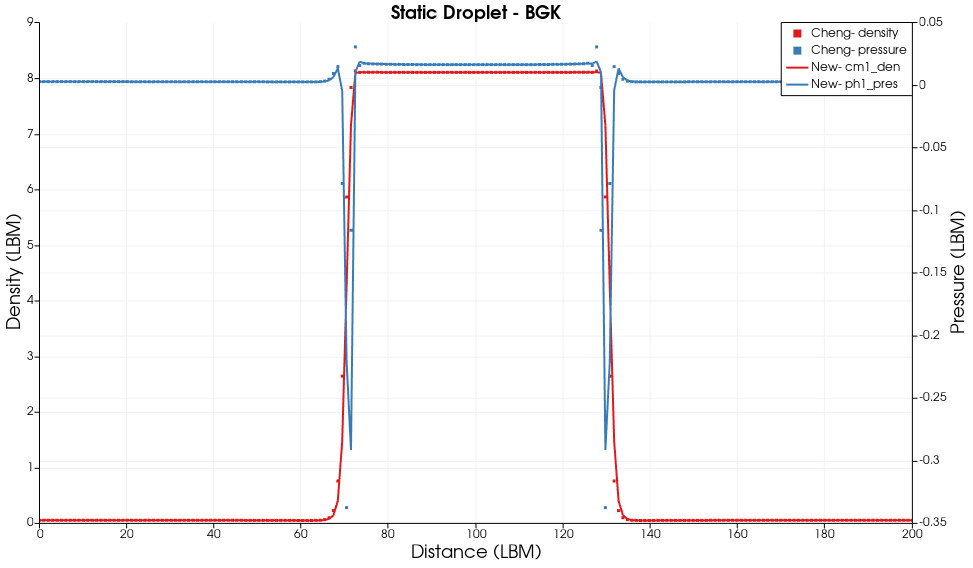
\includegraphics[scale=0.3]{pics/BGK_StaticDroplet.png}
		\caption{Comparison of pressure and density.}
		\label{fig:val1CBGK}
	\end{figure}
	\begin{figure}[h]
		\centering
		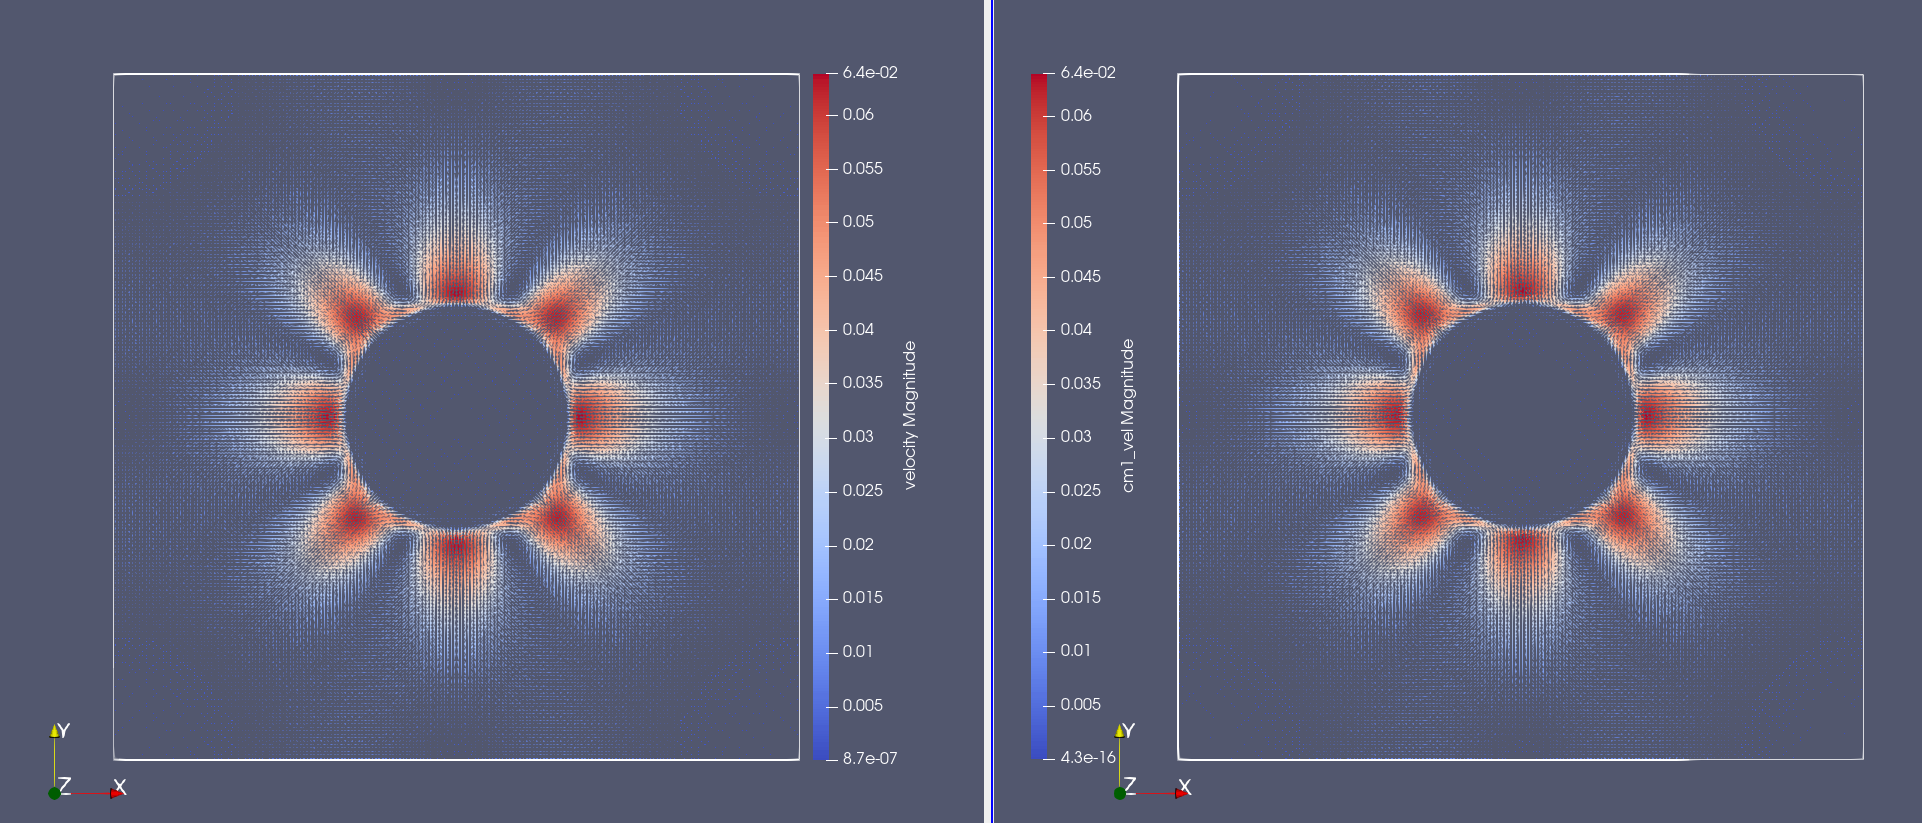
\includegraphics[scale=0.2]{pics/BGK_StaticDroplet_Vel.png}
		\caption{Velocity field.}
		\label{fig:val1CBGKVel}
	\end{figure}

	%\begin{figure}[h]
	%	\centering
	%	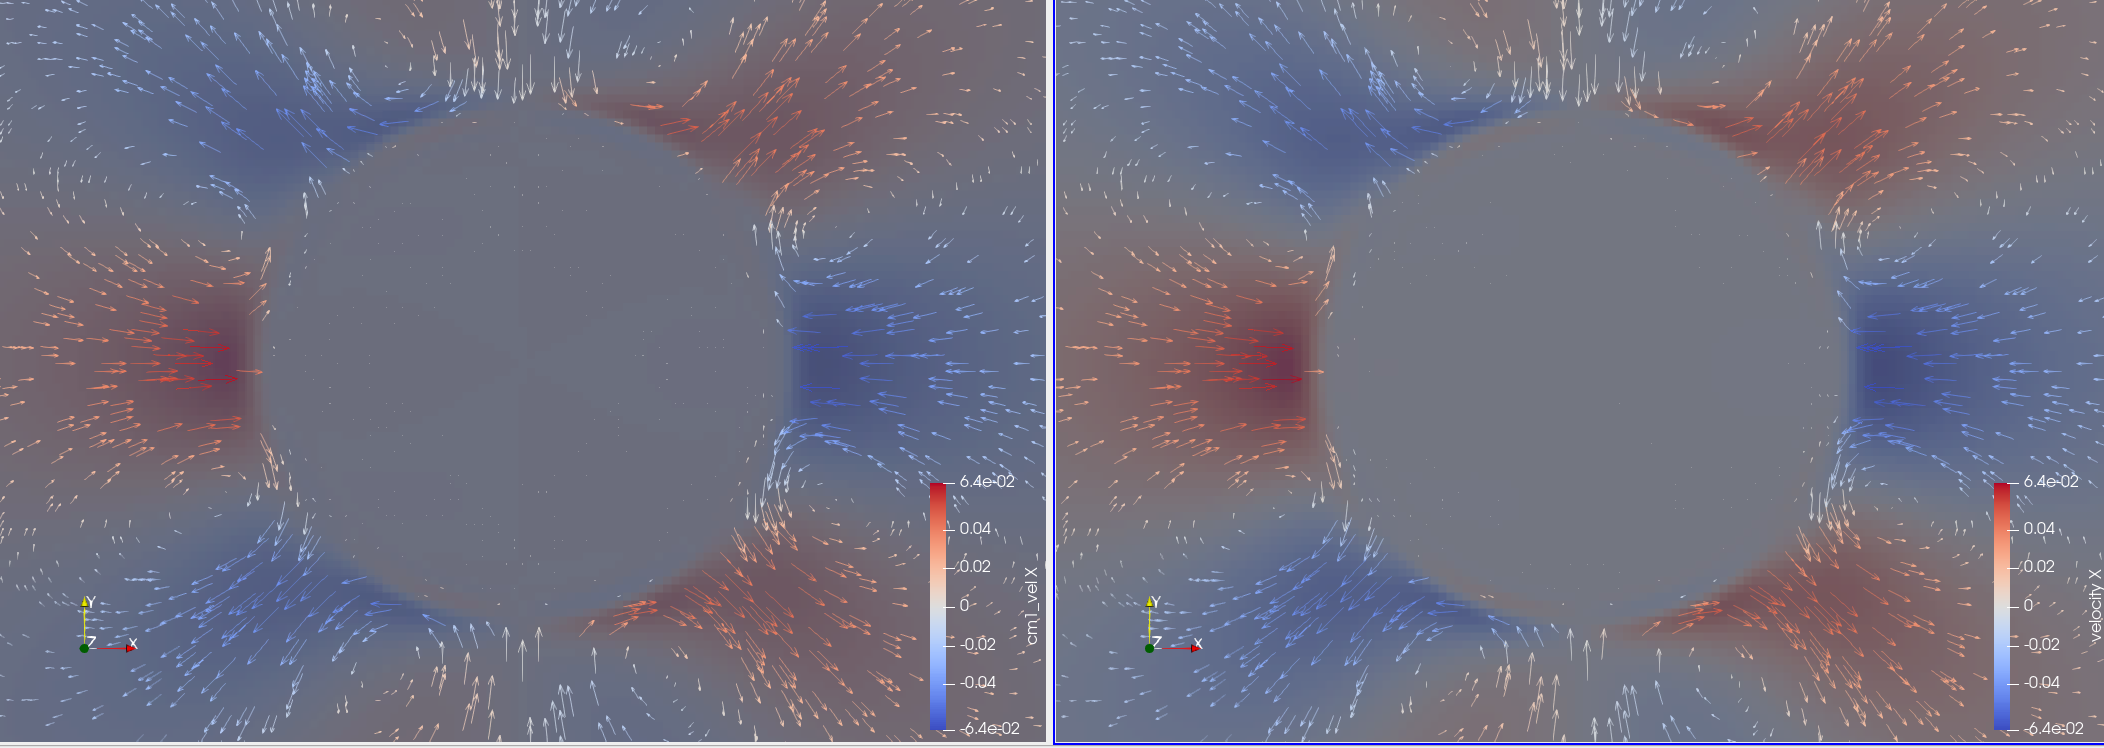
\includegraphics[scale=0.1]{BGK_VelFieldComparison.png}
	%	\caption{Comparison of velocity fields. Close view.}
	%	\label{fig:BGK_VelFieldComparison}
	%\end{figure}
	

	\subsubsection{Single component, MRT, static droplet}
	In folder Oscillating-droplet-single-component, compare Flat Interface and Droplet-Li, as they have different input parameters (structure and calculations are equal). The S vector (-1.d0,-1.d0,-1.d0,-1.d0,-1.5d0,-1.d0,-1.5d0,
	0.d0,0.d0). They run at a new temperature. I have run the Flat Interface, as only input parameters change from the Droplet-Li case. The comparison, now using the MRT case, for the pressure and density profile, is shown in Figure \ref{fig:val1CMRT}. This was not observed for the BGK case, where the velocity vectors point towards the center of the droplet, and then turn up or down in small vortexes.
	\begin{figure}[h]
		\centering
		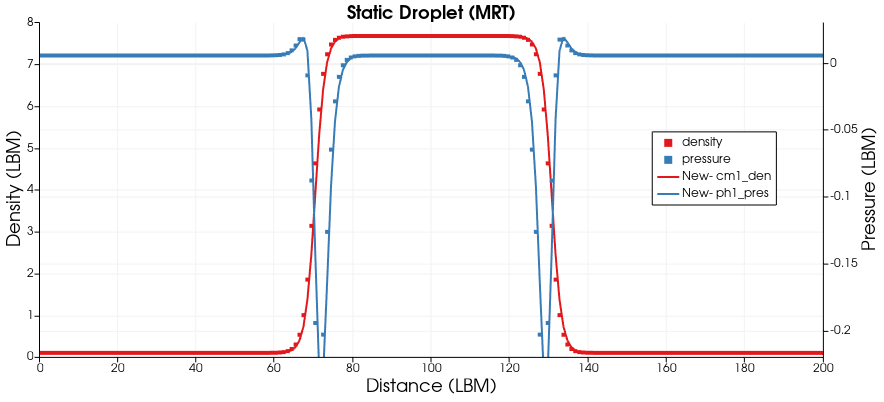
\includegraphics[scale=0.4]{pics/MRT_StaticDroplet_PRho.png}
		\caption{Comparison of pressure and density.}
		\label{fig:val1CMRT}
	\end{figure}
	The velocity field seems to be inverted. In the Cheng's case, the velocity along the X axis, and at the center of the droplet, seems to go away from the droplet. In the new code, this inverts, and the velocity points towards the center of the droplet. This is validated by Figure .
	\begin{figure}[h]
		\centering
		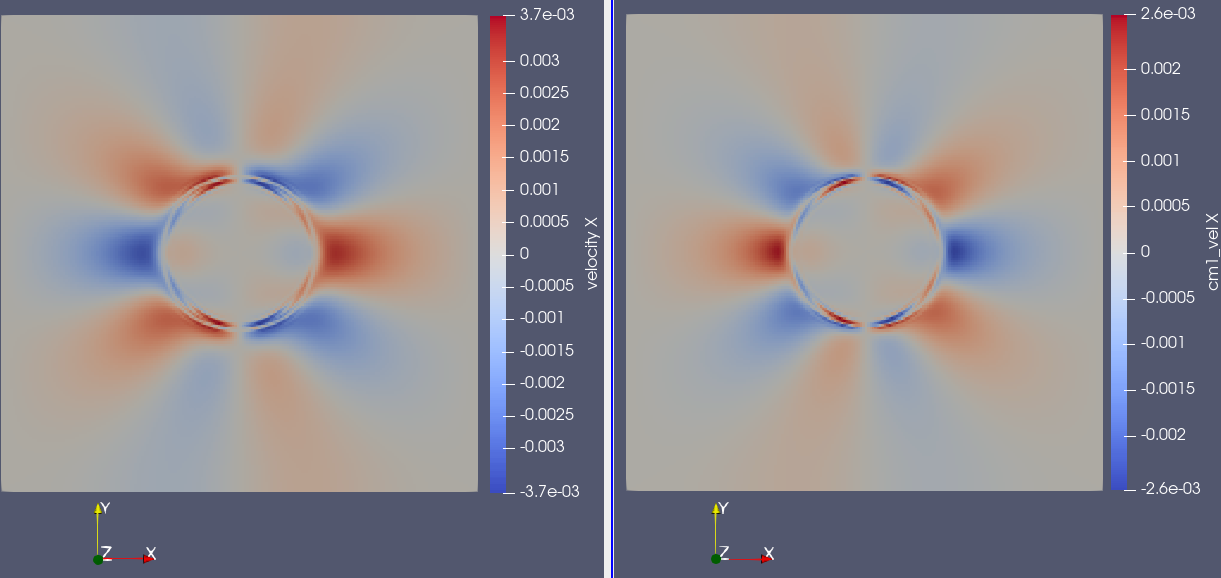
\includegraphics[scale=0.3]{pics/MRT_StaticDroplet_VelField.png}
		\caption{Comparison of pressure and density.}
		\label{fig:MRT_StaticVelField}
	\end{figure}
	\begin{figure}[h]
		\centering
		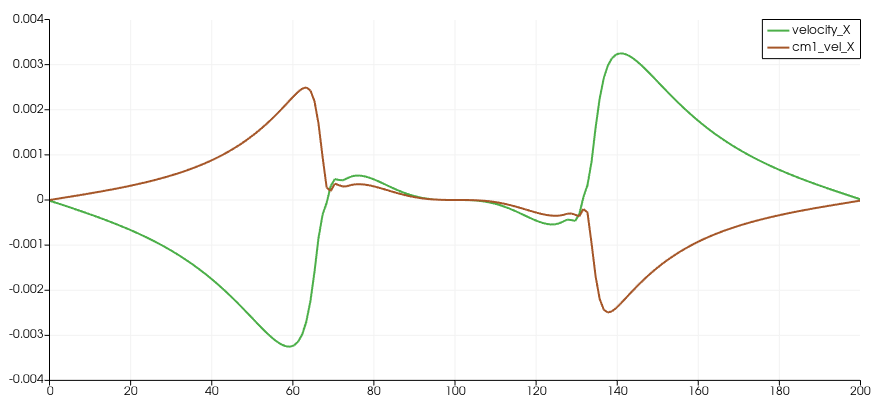
\includegraphics[scale=0.3]{pics/MRT_StaticDroplet_VelProf.png}
		\caption{Comparison of pressure and density.}
		\label{fig:MRT_StaticVelProf}
	\end{figure}
	
	\subsubsection{Single component, BGK, oscillating droplet}
	
	The case was successfully validated. The equilibrium velocity, density, and pressure distribution are depicted, as well as the evolution of the major axis of the droplet against time.
	\begin{figure}[h]
		\centering
		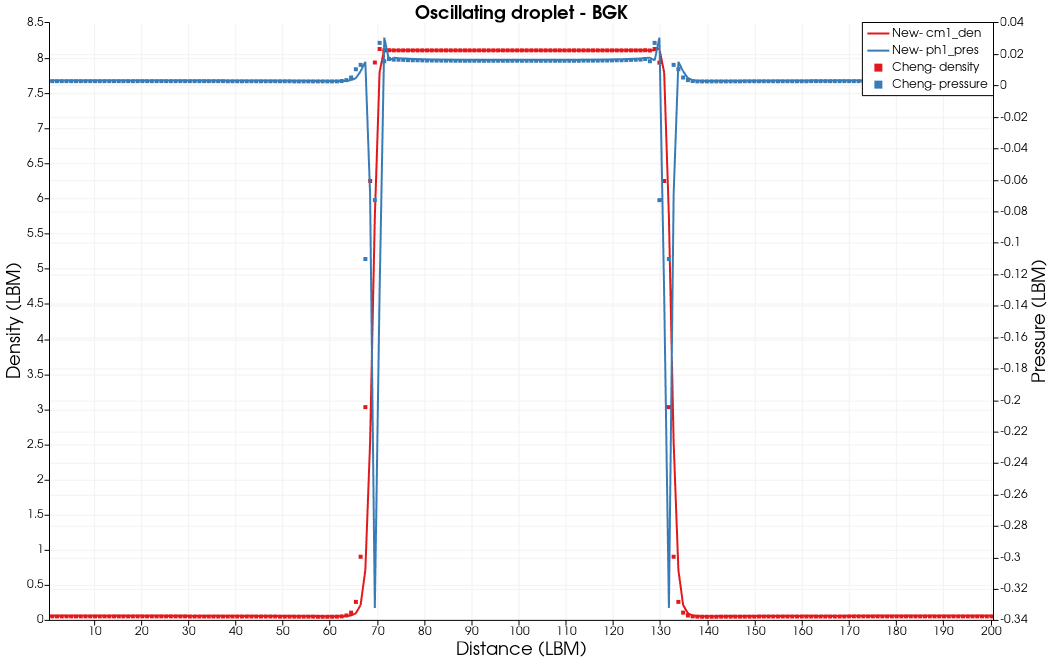
\includegraphics[scale=0.3]{pics/BGK_OscDroplet_PRHO.png}
		\caption{Comparison of pressure and density.}
		\label{fig:val1CBGK_Osc1}
	\end{figure}
	%\begin{figure}[h]
	%	\centering
	%	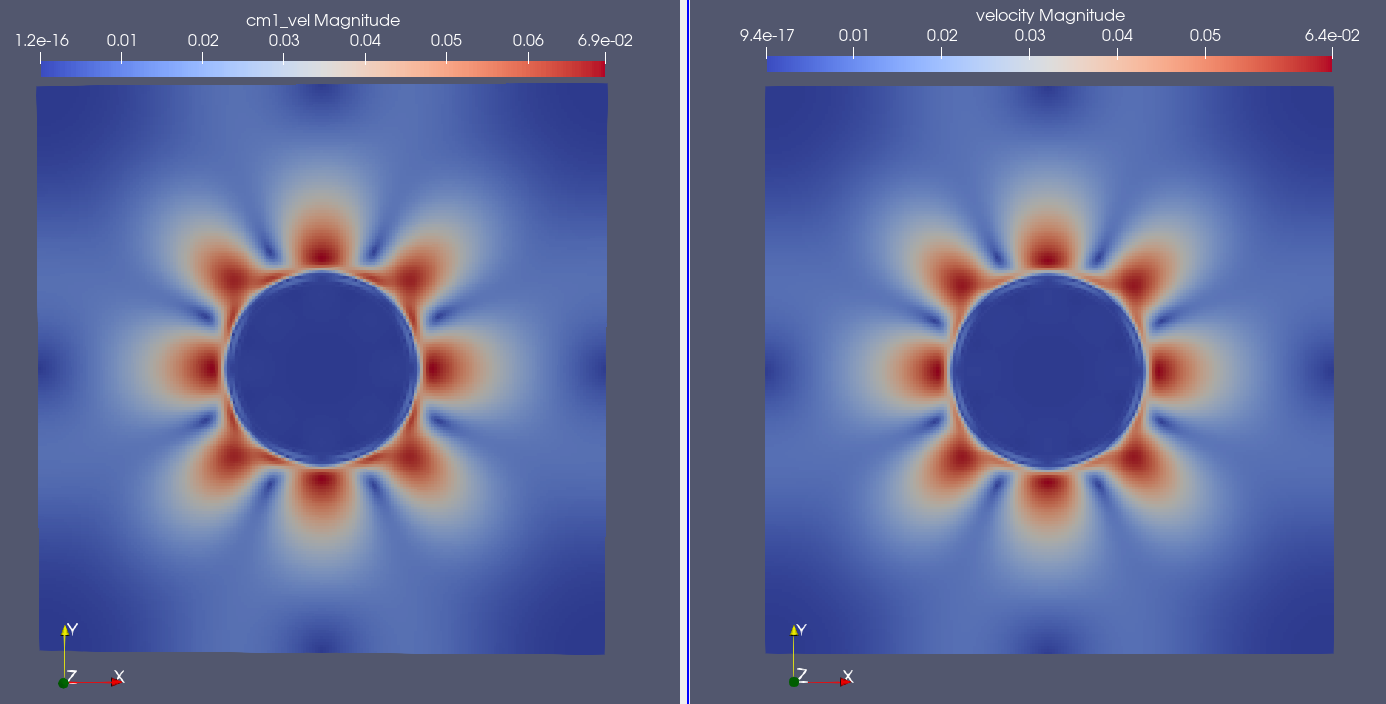
\includegraphics[scale=0.2]{BGK_OscDroplet_VelField.png}
	%	\caption{Velocity field.}
	%	\label{fig:val1CBGK_Osc2}
	%\end{figure}
	\begin{figure}[h]
		\centering
		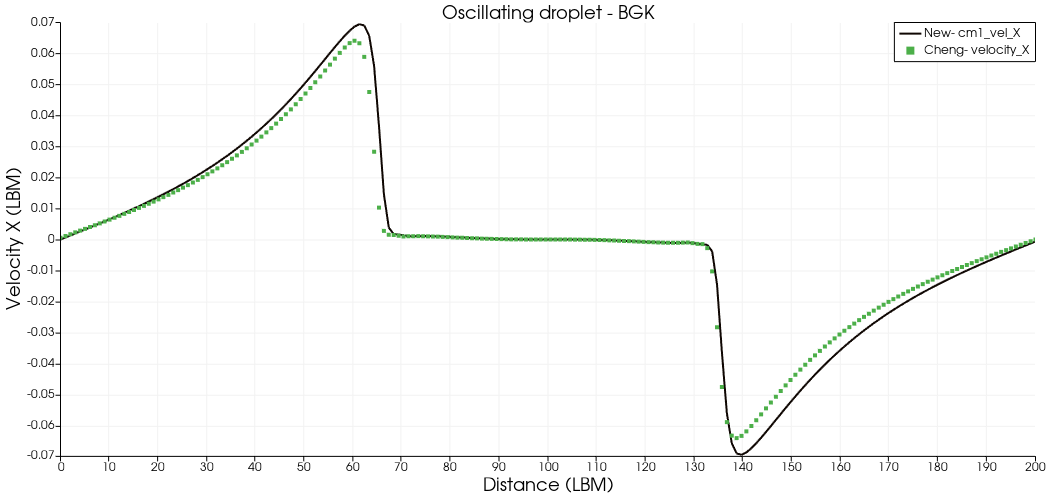
\includegraphics[scale=0.3]{pics/BGK_OscDroplet_VelProf.png}
		\caption{Velocity field.}
		\label{fig:val1CBGK_Osc3}
	\end{figure}
	\begin{figure}[h]
		\centering
		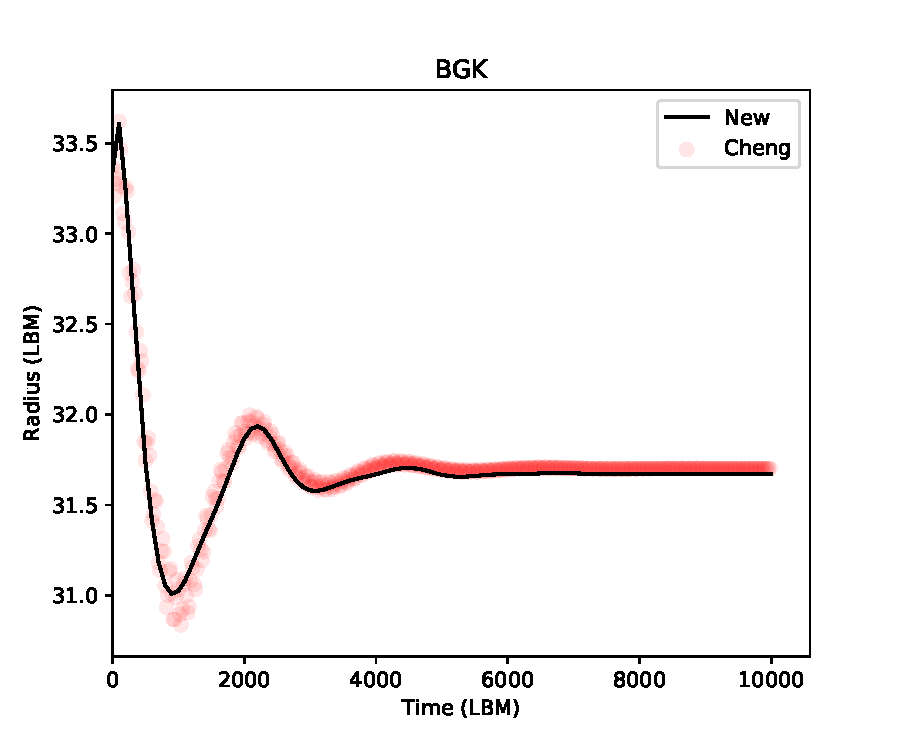
\includegraphics[scale=0.50]{pics/BGKOsc.pdf}
		\caption{Velocity field.}
		\label{fig:val1CBGK_Osc4}
	\end{figure}
	
	\newpage
	\subsubsection{Single component, MRT, oscillating droplet}
	S vector: (-1.0d0,-1.d0,-1.d0,-1.0d0,-1.25d0,-1.0d0,-1.25d0, 0.d0,0.d0). Here changes the width to 8. Cheng's code did not converge for this width, so it was changed back to 5.
	\begin{figure}[h]
		\centering
		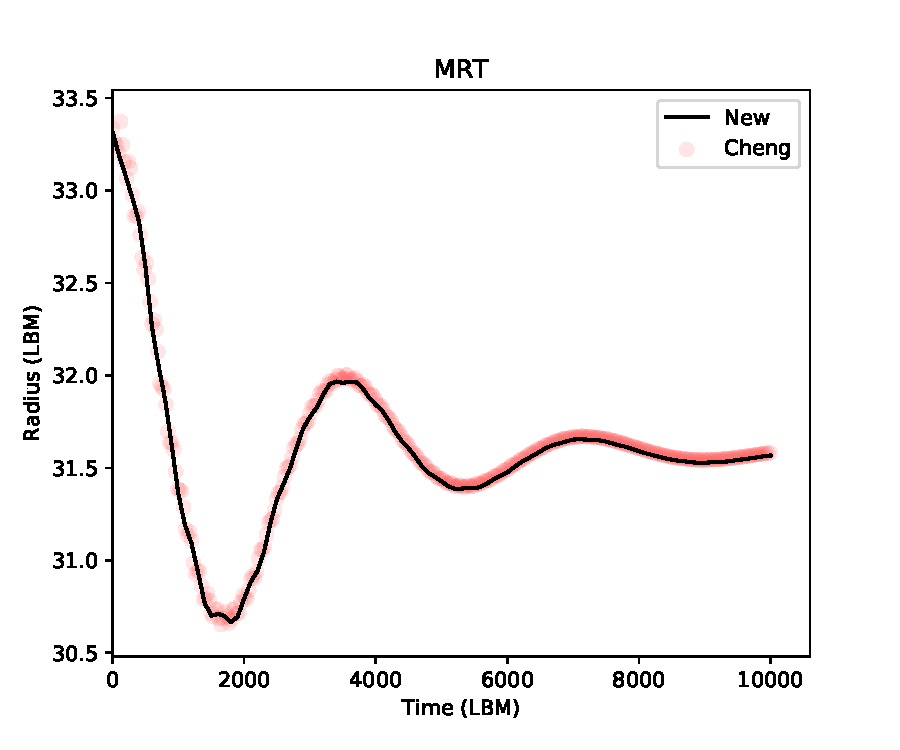
\includegraphics[scale=0.5]{pics/MRTOsc.pdf}
		\caption{Velocity field.}
		\label{fig:MRTOsc}
	\end{figure}
	
	\subsubsection{Single component, MRT, Rotating Droplet}
	
	\subsubsection{Two components, MRT, static droplet}
	Folder Oscillating-droplet. Droplet-suspension-Li-MRT.
	%----------------------------------------------------------------------------------------
	%	SECTION 
	%----------------------------------------------------------------------------------------
	
	\section{Bibliographic Review}


	%----------------------------------------------------------------------------------------
	%	BIBLIOGRAPHY
	%----------------------------------------------------------------------------------------
	\bibliographystyle{apalike}
	\bibliography{ref}
	%----------------------------------------------------------------------------------------
	
	
\end{document}